\begin{frame}{How Symbols get encoded: \alert{Frequency Shift} Chirp Spread Spectrum (\alert{FS-CSS})}
  \alert{Frequency Shift} Chirp Spread Spektrum or \alert{FS-CSS} is used to encode symbols.
  \begin{center}
    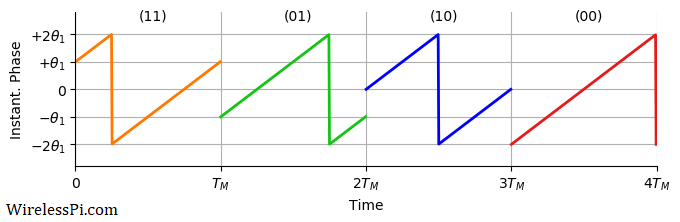
\includegraphics[width=0.55\textwidth]{material/figure-psk-phase-vs-time.png}
  \end{center}
  \alert{The spread factor $SF$} determines the length $\Delta t_c$ of one chirp. $\Delta t_c$ is defined to be proportional to $2^{SF}$. Thus $\Delta t_c \sim 2^{SF}$.
  \begin{center}
    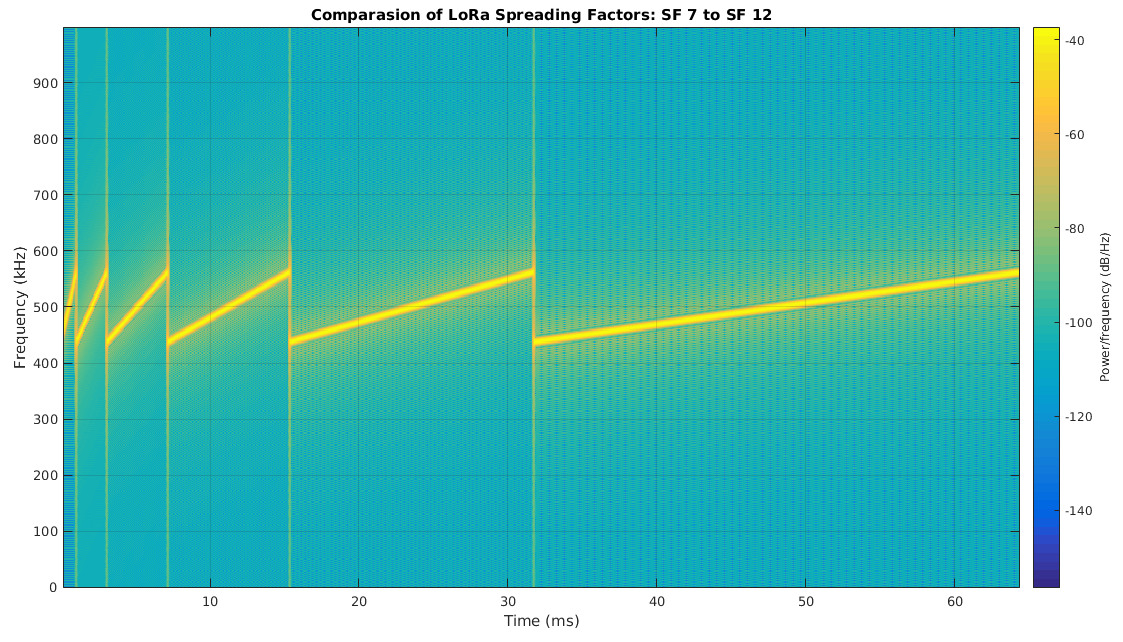
\includegraphics[width=0.3\textwidth]{material/spreading-factor-time-domain.png}
  \end{center}
\end{frame}
